\section{Contenu technique}
	\subsection{Contenu du \og Project Backlog \fg{} initial}
	\begin{longtable}[c]{P{0.05\textwidth}P{0.4\textwidth}P{0.4\textwidth}}
		\caption{Project Backlog pour la partie backend} \\
		\hline
		\bf ID & \bf Titre & \bf Labels \\
		\hline
		\hline
		\csvreader[
			head to column names,
			late after line=\\\\,
			respect leftbrace = false,
			respect rightbrace = false]{Tables/ProjectBacklog_backend.csv}{}%
		{\IssueID & \Title & \Labels}
		\\\hline
	\end{longtable}

	\begin{longtable}[c]{P{0.05\textwidth}P{0.4\textwidth}P{0.4\textwidth}}
		\caption{Project Backlog pour la partie mobile} \\
		\hline
		\bf ID & \bf Titre & \bf Labels \\
		\hline
		\hline
		\csvreader[
			head to column names,
			late after line=\\\\,
			respect leftbrace = false,
			respect rightbrace = false]{Tables/ProjectBacklog_mobile.csv}{}%
		{\IssueID & \Title & \Labels}
		\\\hline
	\end{longtable}


	\subsection{Contenu du backlog du 1\ier{} sprint}
	\subsection{Diagrammes de séquences}
	Lorsque l’utilisateur veut utiliser le service, ce dernier valide son identité auprès du système d'authentification, lequel demande et vérifie avec les serveur CAS les informations de connexion de l'utilisateur.  Le serveur CAS renvoie un \emph{token} qui est remis au service. Pour faire durer la connexion, le système d’authentification gère le \emph{token} CAS comme connexion permanente et renvoie un \emph{token} AUTH  au service. Le service utilise le token AUTH pour vérifier l’identité de l’utilisateur et valider les notifications à émettre. Lorsque le \emph{token} AUTH est valide et qu’une notifications est reçue, la notification est transmise à l’utilisateur. Le diagramme de séquences (figure~\ref{fig.sequences}) illustre ces étapes.
	
	\begin{figure}[hp]
		\centering
		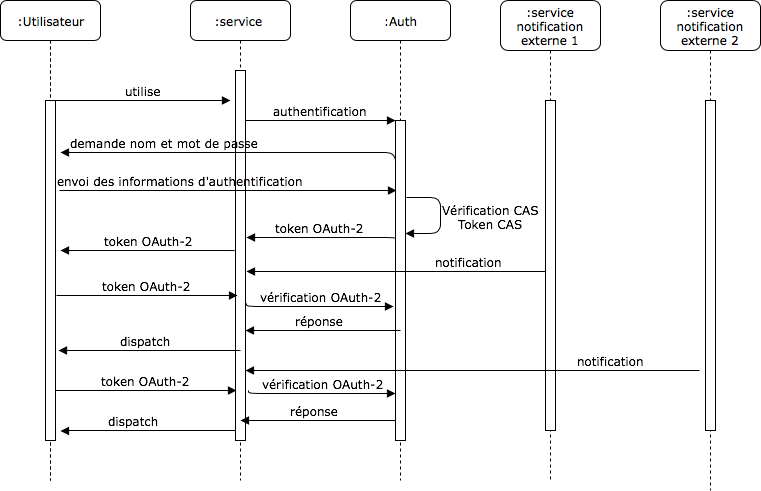
\includegraphics[width=\textwidth]{Figures/Sequences}
		\caption{Diagramme de séquences par rapport à l'authentification à mémoire long terme}
		\label{fig.sequences}
	\end{figure}
	
	\subsection{Architecture du système}
	L’architecture du système (figure~\ref{fig.architecture}) se compose en 4 parties distinctes, soient l’application mobile, le service mobile, l’authentification et le micro-service. Tout d’abord, l’application mobile permettra à un utilisateur d’Android et/ou d’iPhone d’utiliser le service mobile à partir d’une application disponible dans le magasin d’application du téléphone. En ce qui concerne le service mobile, un serveur gérera les notifications du micro-service et des autres équipes de notifications à condition que l’utilisateur soit authentifié. Pour s'authentifier, un utilisateur doit s’authentifier sur le serveur de CAS. Lorsque le token est valide et que les permissions le permettent, des micro-services peuvent être utilisés.
	
	\begin{figure}[hp]
		\centering
		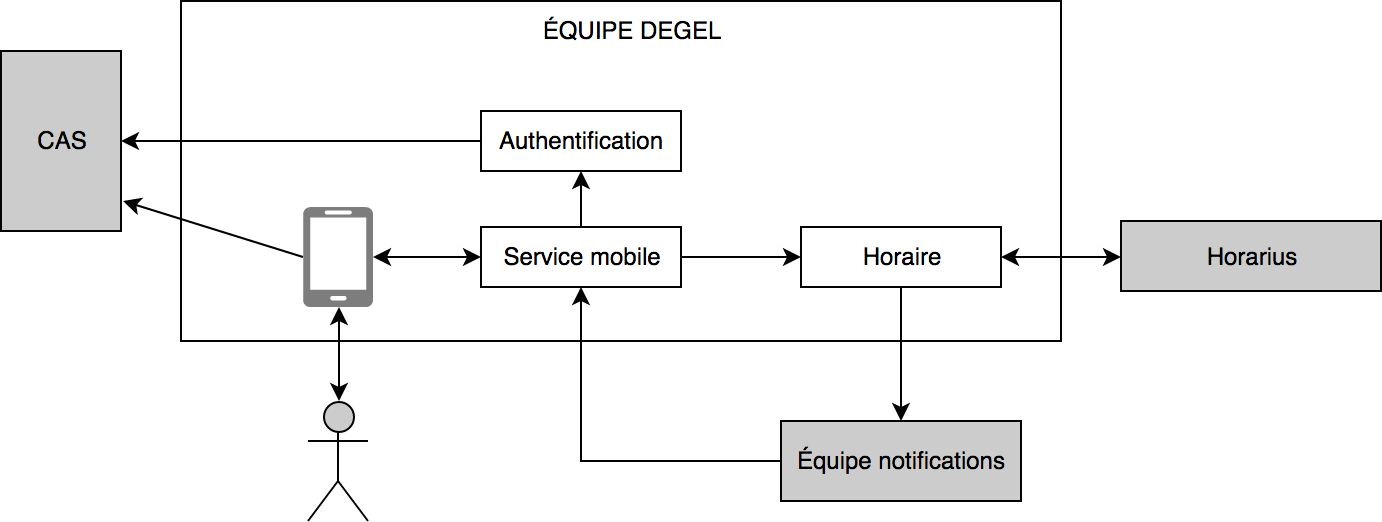
\includegraphics[width=\textwidth]{Figures/Architecture}
		\caption{Architecture du service mobile de notifications pour l’horaire}
		\label{fig.architecture}
	\end{figure}


	\subsection{Modèles de conception}
	Beaucoup de \emph{design patterns} sont abstraits par les \emph{frameworks} qui ont été choisis pour le projet, donc nous nous sommes limités ici à ceux qui seront utilisés explicitement.
	\paragraph{Dependency injection} Le \emph{framework} Spring repose fortement sur l’injection de dépendance et nous l’utiliserons à son maximum. Il suffit d’ajouter l’annotation \code{@AutoWired} à un membre pour indiquer à Spring qu’il doit injecter la valeur et le reste se fait automatiquement.
	\paragraph{Singleton} Dans Spring, ce pattern va de pair avec l’injection de dépendance. En effet, pour injecter la bonne dépendance, Spring recherche une fonction annotée \code{@Bean} qui retourne un objet du bon type. Par défaut, cet objet sera réutilisé pour toutes les injections et est donc de fait un \emph{singleton}.
	\paragraph{MVC} Notre architecture fait un fort usage du \emph{design pattern} MVC. En effet, notre vue est l’application mobile qui ne contient pas de logique d’affaire et communique avec les contrôleurs du \emph{backend} avec des modèles précis sérialisés en JSON. 